% Created 2013-07-29 Mon 20:04
\documentclass[a4paper,11pt]{article}
\listfiles
\usepackage[T1]{fontenc}
\usepackage{hyperref}
\tolerance=1000
\usepackage{fontspec}
\usepackage{biblatex}
\usepackage{graphicx}
\usepackage{fullpage}
\usepackage{caption}
\usepackage{subfig}
\usepackage{hyperref}
\usepackage{moreverb}
\usepackage{fancyvrb}
\usepackage[ruled]{algorithm2e}
\usepackage{cuted}

\bibliography{report}
\defaultfontfeatures{Mapping=tex-text}
\setromanfont[Ligatures={Common},Numbers={Lining}]{Linux Libertine}
%\setmonofont{Liberation Mono}   

\newsavebox{\boxone}
\newsavebox{\boxtwo}
\newsavebox{\boxthree}
\newsavebox{\boxfour}

\title{Sokoban: Search in a complex domain}
\author{Yann Chazallon,  Nicolas Dossou-Gb{\'e}t{\'e}, Tony Chan Ki Hong and Michal Staniaszek}
\date{\today}

\begin{document}

\maketitle

\begin{abstract}
  In this report we describe our implementation of a \emph{Sokoban} solver. We
  use a two stage method to find the solution. A bi-directional best-first
  search with the \textbf{\emph{HEURISTIC IMPLEMENTATION}} as a heuristic is
  used to find the path of boxes on the map. This disjoint path is then linked
  by using A* to find the path between successive box moves. The solver is
  currently able to solve 47 of the 100 evaluation maps on Kattis, and 75 of the
  100 maps in the simpler test set within the 11 second time limit.
\end{abstract}

\begin{figure}[!ht]
  \captionsetup[subfigure]{labelformat=empty}
  \centering
  \subfloat[][\centering Yann Chazallon\\ 91/01/16]{
    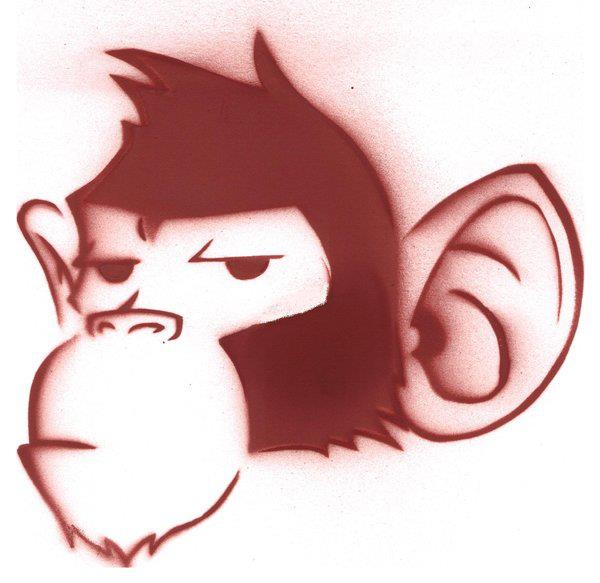
\includegraphics[width=.2\textwidth]{img/yann.jpg}
  }\quad
  \subfloat[][\centering Nicolas Dossou-Gb{\'e}t{\'e}\\ 89/09/26]{
    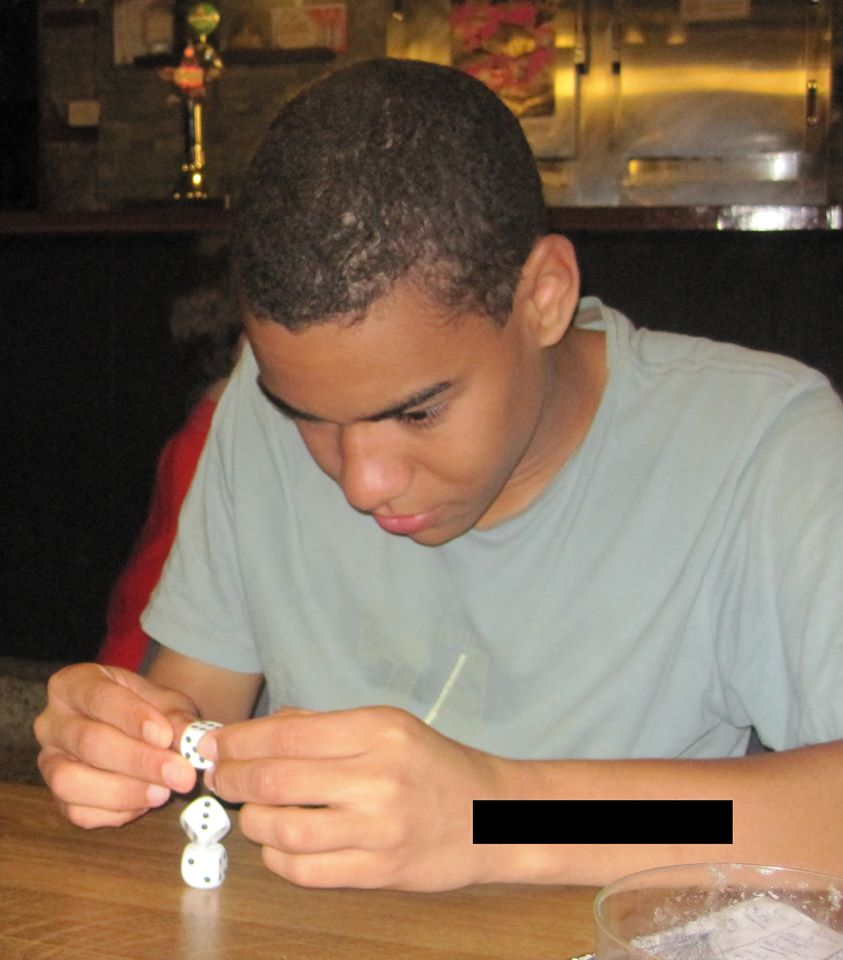
\includegraphics[width=.2\textwidth]{img/nicolas.jpg}
  }\quad
  \subfloat[][\centering Tony Chan Ki Hong\\ 92/07/25]{
    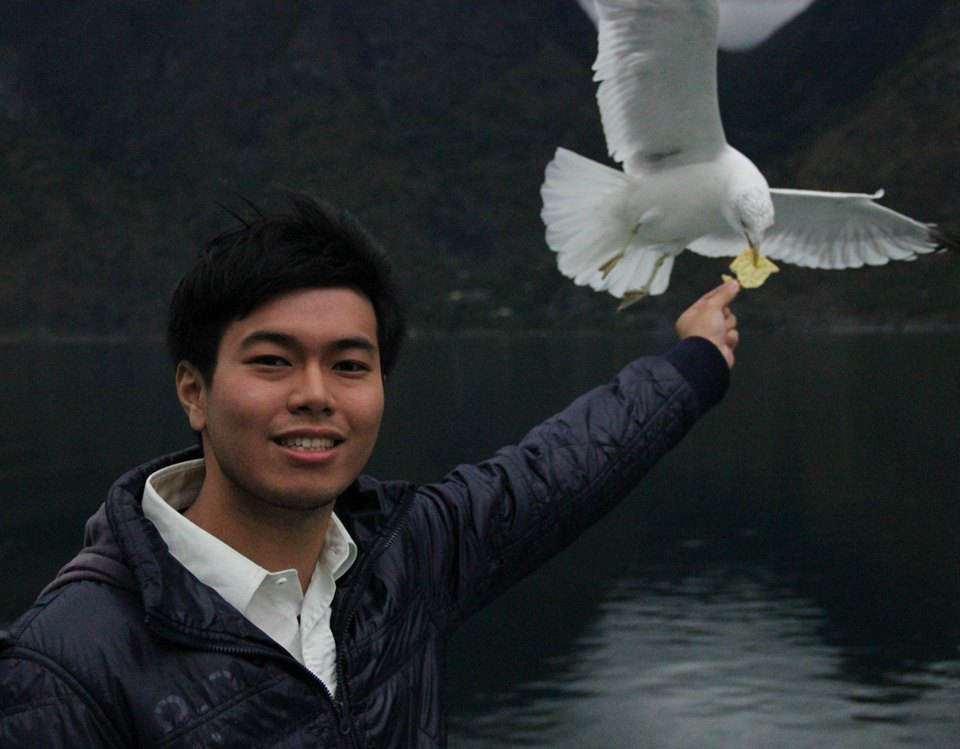
\includegraphics[width=.2\textwidth]{img/tony.jpg}
  }\quad
  \subfloat[][\centering Michal Staniaszek\\ 90/12/07]{
    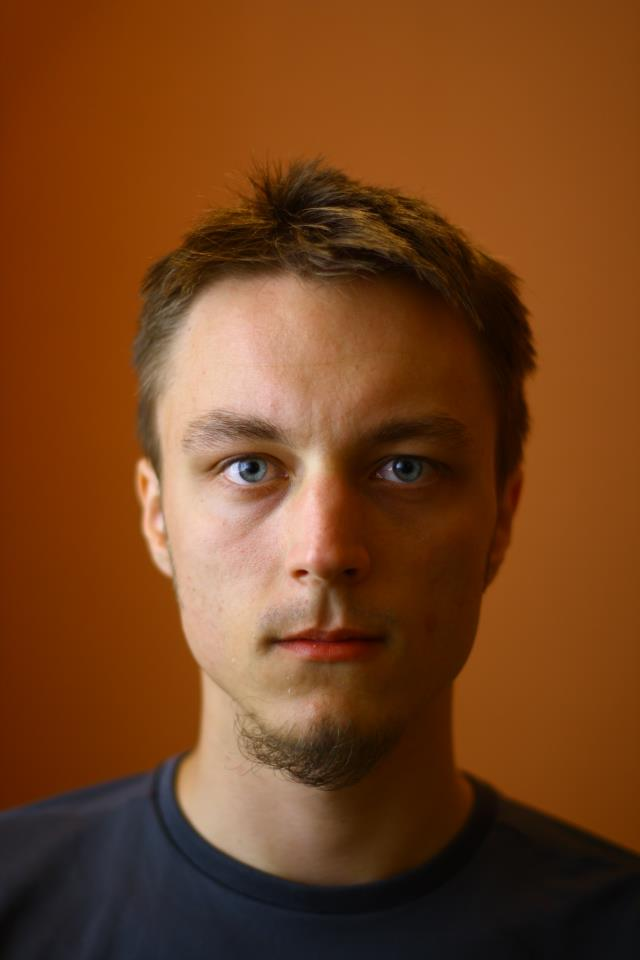
\includegraphics[width=.2\textwidth]{img/michal.jpg}
  }
\end{figure}

\section{Introduction}
\emph{Sokoban} is a puzzle game which written in 1981 by Hiroyuki
Imabayashi. First published in 1982, it is now a very popular game, with many
clones available on the internet. The player controls a warehouse keeper (for
which \emph{sokoban} is the Japanese word), whose job it is to push boxes onto
goal locations on the map. The player can move in four directions (up, down,
left or right) on the map, which is split into discrete cells. The player can
push boxes, but is unable to pull them. To be able to push a box, the player
must be adjacent to it, and there must be an empty space behind the box into
which it can be pushed. Only one box can be moved at a time; if two boxes are
contacting each other, pushing one box does not move the other. While there are
many graphical implementations, there are also many text-based implementations
which use symbols for representing parts of the board, an example of which is
shown in Figure \ref{fig:mapex}.

\begin{lrbox}{\boxone}
  \begin{minipage}{.25\textwidth}
\centering
\begin{BVerbatim}
#######
#  .@ #
# #.# #
#   $ #
#.$$ ##
#  ###
####
\end{BVerbatim}
  \end{minipage}
\end{lrbox}%

\begin{lrbox}{\boxtwo}
  \begin{minipage}{.25\textwidth}
\centering
\begin{BVerbatim}
#######
#  .@ #
# #.# #
# $$  #
#*   ##
#  ###
####
\end{BVerbatim}
  \end{minipage}
\end{lrbox}%

\begin{lrbox}{\boxthree}
  \begin{minipage}{.25\textwidth}
\centering
\begin{BVerbatim}
#######
#  .@ #
# #.# #
#$ $  #
#*   ##
#  ###
####
\end{BVerbatim}
  \end{minipage}
\end{lrbox}%

\begin{lrbox}{\boxfour}
  \begin{minipage}{.25\textwidth}
\centering
\begin{BVerbatim}
#######
#  *  #
# #*# #
#  @  #
#*   ##
#  ###
####
\end{BVerbatim}
  \end{minipage}
\end{lrbox}%

\begin{figure*}
  \subfloat[A basic map]{\usebox{\boxone}}
  \subfloat[Half solved]{\usebox{\boxtwo}}
  \subfloat[In an unsolvable state]{\usebox{\boxthree}}
  \subfloat[The solved map]{\usebox{\boxfour}}
  \caption{A typical \emph{Sokoban} map. The player is represented by \texttt{@}, or \texttt{+} when on a goal, boxes by \texttt{\$} or \texttt{*} on a goal, walls by \texttt{\#}, goals by a period, and empty space by a blank. The map in (c) is unsolvable, as the two boxes on the left are both against a wall. This is called a \emph{deadlock}.}
  \label{fig:mapex}
\end{figure*}

The game has garnered some interest in the artificial intelligence (AI)
community due to the difficulty of finding automatic solutions. Games are an
ideal platform for the development and testing of AI techniques, as game
environments are much simpler and less (or not at all) noisy, and also have sets
of simple rules for interaction with the world. Working in such environments
allows for more control and closer investigation of the relevant parts of the
problem that is being considered. \emph{Sokoban} in particular is an interesting
problem due to its high branching factor, and the depth of the search trees that
are generated when attempting to solve a problem. Even relatively simple
problems can take upwards of 100 moves to solve, and more complex problems can
exceed 500 moves, even in the optimal case. Additionally, it is possible to
extend the search tree indefinitely---there is no time limit, and boxes can be
pushed without restraint, so long as the push is valid. The branching factor is
the total number of valid actions that can be applied to any box reachable from
the player's current position. In the worst case, if there are $N$ boxes, all of
which are accessible and can be pushed in any direction, the factor is $4N$
(each box can be pushed in 4 directions). Although in practice it is not
possible to access all boxes, or push them in an arbitrary direction, but most
maps have a large enough number of boxes that the branching factor has a large
impact on the number of states expanded.

\section{Method}

The solver should be able to read string-based map representations into a
manipulable object. It must be possible to move boxes and the player on this map
representation. In addition, the solver must be able to deal with both static
and dynamic deadlocks. A heuristic is required to drive the search towards the
goal. Finally, a search method is required, which, given a start and goal state,
must be able to find a path between the states, or indicate that a path does not
exist.

\subsection{Map Representation}

To be able to solve a \emph{Sokoban} map, it is necessary to have a map
representation which can be manipulated and used to gain information about the
state of the board. The representation of the state is required by any search
method in order to be able to generate successor states and find a path to the
goal state. Our map representation uses a two-level model, where dynamic objects
(boxes and the player) are separated from the static part of the map, that is,
the goals, empty space, and walls. By separating these two parts of the map, we
are able to reduce the storage space required for each board, as the static map
is represented only once. When move validity must be checked, the dynamic
objects are ``collapsed'' onto the static map.

The static map also stores a costmap which relates each position on the board to
a set of costs to reach each goal. The costmap is calculated by doing a flood
fill which attempts to pull a single box from each goal to all points on the
map, with no other boxes present. This gives an optimistic estimate of the
number of steps required to move a box from any position on the map to any goal
when the map is populated with boxes, as in practice the path of the box may be
obstructed by other boxes.

Functionality for checking board equality is also required to be able to perform
search, as it is necessary to check whether states have been visited previously
in order to prevent unnecessary re-evaluation of states. Our map representation
has different types of equality based on the state expansion procedure being
used.

The state expansion defines how successors of a given state are generated. The
player space expansion is based on the motion of the player alone; the player
can move up, down, left or right, and so the maximum number of successors is
4. In this expansion, exact equality is used---the position of all dynamic
objects on the board is checked, and the player and all boxes must be in exactly
the same locations for the boards to be equal.

The board space expansion is based on the motion of all boxes in the state. With
this expansion, the maximum number of successors is $4M$, where $M$ is the
number of boxes which can be reached by the player, as each box could be pushed
in one of four possible directions. To determine the successor states of this
state, it is first necessary to find all the positions which are accessible by
the player. This is done by starting a flood fill from the current player
position and finding points at which a box can be accessed. With this expansion,
the board equality no longer checks the exact location of the player. Instead,
the top leftmost position accessible by the player is used to represent the
player. This means that states in which the player has the same accessible area,
and where boxes are in the same positions are considered equal.

hashing!

\subsection{Deadlock Detection}
The exists of Deadlock makes Sokoban even more hard to solve. As Player cannot
pull a box, sometimes player may pushes the box into a position that the box can
never reach the goal.

Static Lock

The meaning of static lock is that we cannot never push the box to the goal even
without other boxes.

While recieving the map, the program will try to put a box on each goal and
check the points that is reachable by the box by pull (i.e. do a BFS for each
goal with reverse action). Reachable points are stored in a map for each
goal. The cost for a box at Non-reachable points to a specific goal will be
Positive infinity.

Dynamic Lock

In this case, the point of a box is supposed to be reachable to some specific
goal. However, there are some boxes blocking in the middle and it is impossible
to remove that blocking box.

\subsection{Heuristics}

\subsection{Search Method}
The search methods form the core of the solver. Using them, we find a path
between a starting board state and the goal state, where all boxes are on
goals. We implemented three different search methods; A*, best-first search and
bi-directional search. A* expands nodes in a specific order based on the value
of a state evaluation function $f(s)=g(s)+h(s)$, where $s$ is some board
state. The value $h(s)$ is the heuristic value of the state, and represents an
estimate of how far the state $s$ is from the goal. The value of $g(s)$ depends
on the path that was taken to reach this node---the longer the path, the higher
the value. A* places states into a priority queue and expands them starting from
nodes with a lower $f$ value; a shorter distance to the goal. This evaluation
function means that so long as $h(s)$ is an underestimate (an \emph{admissible}
heuristic) of the true cost to the goal state, A* is both optimal and complete,
that is, it will always find a solution if one exists, and that solution will be
optimal\cite{aima}.

In best-first search, the cost to reach the current node is not considered in
the expansion, and so the evaluation function simplifies to $f(s)=h(s)$. This
results in the search always expanding the state with the lowest cost to the
goal, regardless of how far it is from the start state. This results in a loss
of optimality and completeness \cite{aima}, but can lead to a goal being found
much faster than in the case of A*. Since we do not care about finding an
optimal solution, and speed is of the essence in this problem, best-first search
is more appropriate than A*. Our implementation is shown in Figure
\ref{alg:bestfirst}.

To further improve the speed of the search, we implemented a bi-directional
search. While both A* and best-first search have a complexity of
$\mathcal{O}(b^d)$, running two searches, one from the start state to the goal,
and one from the goal state to the start, reduces this to $\mathcal{O}(b^{d/2})$
\cite{aima}, where $b$ is the branching factor, and $d$ is the solution
depth. The search terminates when the frontiers of the two searches meet. This
can be understood intuitively by considering a circle centred on the front node,
with a radius $d$, with the goal node on the edge of the circle. The area inside
this circle is very large compared to two smaller circles centred on the start
and the goal meeting in the middle. Our implementation of bi-directional search
is shown in Figure \ref{alg:bidi}.

Our approach involves splitting the problem into two distinct search
problems. First, we find the actions required to move the boxes from the start
state to the goal state using a best-first bi-directional search. Once this
intermediate path has been found, we run a series of A* searches to find the
path of the player between each successive box movement, which gives us the
final path from the start to the goal. When finding the player path, we consider
boxes as immovable objects.

\begin{algorithm}
  \DontPrintSemicolon
  \SetKwProg{Fn}{Function}{}{end}
  \SetKwInOut{Input}{input}\SetKwInOut{Output}{output}
  \Input{An open list $O$, containing a start node $S$. A goal node $G$. A closed list $C$.}
  \Output{A list of action, point tuples $(A,P)$, containing the path from $S$ to $G$.}
  \Fn{findPath()}{
    \While{$O \neq \emptyset$}{
      successors $=$ step()\;
      \lIf{$G \in $ successors}{\Return successors.get($G$).unwind()}
    }
  }
  \Fn{step()}{
    front $=$ open.front()\;
    successors $=$ front.expand()\;
    closed.add(front)\;
    \ForEach{$n \in $ successors}{
      \If{$n \notin C \land n \notin O$}{
        \tcp{nodes in $O$ sorted by heuristic value}
        $n$.costEstimate $=$ h($n$.state, $G$)\;
        $O$.add($n$)\;
      }
    }
    \Return successors\;
  }
\caption{Best-first search}
\label{alg:bestfirst}
\end{algorithm}

\section{Implementation}
In our implementation, we use several objects which allow for cleaner code and
easier access to required data. The most basic part of the implementation is the
\texttt{Board} class, which holds methods to deal with moving the player and
accessing various information about the state of the board. The \texttt{Board}
object holds a list of dynamic points, as well as a reference to the static
map. The static map is implemented as a singleton, so all objects created have a
reference to that same object. This reduces memory usage, as the static part of
the map is not duplicated for each \texttt{Board} object.

As we are using bi-directional search, the search methods have been implemented
in a way that allows their usage in both a bi-directional and a single
directional search. This is important as we do not perform only a single search
to find the path to the goal. To achieve this, we use a \texttt{step} method to
perform a single step of the search. This step, in the case of A* and best-first
search, is to expand the front of the priority queue, and add the successors to
the open lists, performing any relevant checks. The best-first search
implementation is shown in Algorithm \ref{alg:bestfirst}. Algorithm
\ref{alg:bidi} shows our implementation of bi-directional search, which makes
use of best-first search.

The search methods make use of a custom \texttt{SearchNode} class, which stores
a parent node, a \texttt{Board} representing the state of that node, and a
\texttt{BoardAction} object, which represents the action used to generate the
board by a point object (the location of the pushed box) and an associated
\texttt{Action} enum, which is one of $\{up, down, left, right\}$, and indicates
the direction of the push. The \texttt{unwind} method of the \texttt{SearchNode}
recurses up to the start node, and reconstructs the path from there to the node
on which the method was called.

\begin{algorithm}
  \DontPrintSemicolon
  \KwData{Search implementations forwards and backwards, initialised with start and goal.}
  \KwResult{A list of tuples of (\texttt{point}, \texttt{int}) containing motion of boxes from start to goal.}

  \Begin{
    current $\longleftarrow$ forwards\;
    opposite $\longleftarrow$ backwards\;
    new $\longleftarrow \emptyset$\;
    key $\longleftarrow $ \texttt{null}\;
    \Repeat{key $\neq$ \texttt{null}}{
      swap current and opposite\;
      new $\longleftarrow$ current.step()\;
      \lIf{node $\in$ new $\land$ node $\in$ opposite.open}{key $\longleftarrow$ node}
    }
    fkey $\longleftarrow$ forwards.open.get(key)\;
    bkey $\longleftarrow$ backwards.open.get(key)\;
    fActions $\longleftarrow$ fkey.unwind()\;
    bActions $\longleftarrow$ bkey.unwind()\;
    \Return merge(fActions, bActions.reverse())\;
  }
\caption{Bi-directional search}
\label{alg:bidi}
\end{algorithm}


\begin{algorithm}
  \DontPrintSemicolon
  \SetKwProg{Fn}{Function}{}{end}
  \SetKwInOut{Input}{input}\SetKwInOut{Output}{output}
  \Input{A box position $B$.}
  \Output{A boolean representing whether or not the box at point $B$ is locked.}
  \If{B is on goal}{
    \Return false
  }
  closed $\longleftarrow \emptyset$
  \return isMovable($B$, $closed$)

  \Fn{isMovable(Point $P$, Set $closed$)}{
    \If{$P =$ WALL}
      \Return false
    \ElseIf{$P =$ BOX}{
      \If{$P \in closed$}{
	closed.add(P)\;
	\Return false
      }\Else{
      \Return ((isMovable(P.left, closed) \and (isMovable(P.right, closed)) \or ((isMovable(P.up, closed) \and (isMovable(P.down, closed))
      }
    }\Else{
       \Return true
    }
  }
\caption{Single box dynamic lock detection}
\label{alg:singledynamiclock}
\end{algorithm}

\section{Evaluation}
experimental evaluation and a thorough analysis of your results. This section should include:
How well did your agent do on the different maps?
\begin{figure}
  \centering

  \caption{timing for experimental results}
  \label{fig:exptime}
\end{figure}
\section{Discussion}
During our first meeting, we discussed several ideas about how to solve the
problem, based on brief readings of some previous work \cite{virkkala, jung}. We
decided that in the ideal case we should attempt to implement some of the
techniques mentioned in these papers to produce an effective solver. The first
step we too was to create the foundations for the solver, by implementing a
board representation and some search algorithms, which we knew we would need
based on our discussions. Work was distributed by each group member choosing
something to work on, and then working on the parts of the solver related to
that. This worked reasonably well, but meant that some members did not fully
understand the code that was being used, because they had no part in writing
it. We attempted to amend this by commenting methods with enough information to
understand what the method was \emph{supposed} to do. In order to check that
important methods were doing what they were supposed to be doing, we used JUnit
tests, running them whenever there were significant changes to the code to
ensure that everything was working as expected.

Our approach to developing the solver led to some problems. Because each member
was working on a somewhat different task, we did not meet directly very often,
which resulted in too little communication and only a vague idea of what we were
aiming for. As such, we spent the first couple of weeks adding unnecessary code
to the solver, which would be removed later. This left us with a solver which,
at the milestone deadline, could solve the four basic maps, but nothing
else. Once we started meeting more often, we were able to make progress on the
solver, but most of the progress was fixing errors that were caused by
misunderstandings of the intended use of methods, and various other bugs which
could not be directly detected by the unit tests. Fixing these problems left us
with little time to consider any more complex techniques that we could use to
improve the solver, which negatively impacted on the final result.

Our first approach to the problem was to use the motion of the player as the
state expansion in an A* search implementation. This solver was able to complete
very simple maps, but the size of the search space was far too large to solve
any of the maps in the test set. Our second attempt was to use an expansion
which considered all valid moves of boxes in a given board state. This reduced
the search space to only those moves which were relevant to solving the
problem. Once all bugs had been fixed, this version of the solver could solve a
small number of maps in the test set, but continued to be hampered by
slowness. This version was improved by using a more efficient equality check
based on a string representation of the board, and a best-first search
implementation. With this, we were able to solve approximately 15 of the maps
from the online test set. Our current approach was reached by our need to
improve the speed of the algorithm, and we thought that rather than using
improved heuristics, changing the search algorithm would be more effective. We
implemented a minimum matching heuristic, but the additional complexity resulted
in the search taking longer despite the improved heuristic estimates. The
performance measure used during the process was the number of maps of the Kattis
test set solved by the solver. Profiling was also used to judge the effects of
more efficient implementations of parts of the solver.

How would you solve it if you were asked to do it again given what you know now?

\printbibliography

\end{document}